%-----------------------------------------------------------------------------
%
%               Template for sigplanconf LaTeX Class
%
% Name:         sigplanconf-template.tex
%
% Purpose:      A template for sigplanconf.cls, which is a LaTeX 2e class
%               file for SIGPLAN conference proceedings.
%
% Guide:        Refer to "Author's Guide to the ACM SIGPLAN Class,"
%               sigplanconf-guide.pdf
%
% Author:       Paul C. Anagnostopoulos
%               Windfall Software
%               978 371-2316
%               paul@windfall.com
%
% Created:      15 February 2005
%
%-----------------------------------------------------------------------------


\documentclass{sigplanconf}

% The following \documentclass options may be useful:

% preprint      Remove this option only once the paper is in final form.
% 10pt          To set in 10-point type instead of 9-point.
% 11pt          To set in 11-point type instead of 9-point.
% authoryear    To obtain author/year citation style instead of numeric.

\usepackage{pslatex}
\usepackage{hyperref}
\usepackage{url,moreverb,graphicx}
\usepackage{ifthen}
\usepackage{amssymb}
\usepackage{listings}
\usepackage{xspace}
\usepackage{rotating}
\usepackage{fixmath}
%\usepackage{relsize}
\usepackage{mdwlist}
%\usepackage{enumitem}
%\usepackage{paralist}
\usepackage{pseudocode}
\usepackage[lined,boxruled]{algorithm2e}
%\usepackage{algorithm2e}
\usepackage{theorem}
\usepackage{amsmath}
\usepackage{comment}
\usepackage{multirow}
 \let\labelindent\relax
\usepackage{enumitem}
%\setlist[itemize]{noitemsep}
%\setlist[description]{noitemsep}
%\setlist[enumerate]{noitemsep}

\usepackage{float}
%\usepackage{floatflt}
%\usepackage[small,it]{caption} %reduces the size of captions under tables and figures.
\usepackage{subfigure}
%\usepackage{fancybox}
\usepackage{mdframed}
\usepackage{shadow}
\usepackage{balance}
\usepackage{pifont}% http://ctan.org/pkg/pifont
\newcommand{\cmark}{\ding{51}\xspace}%
\newcommand{\xmark}{\ding{55}\xspace}%

\usepackage{color}
\usepackage{textcomp}

\usepackage{quoting}



\begin{document}

\special{papersize=8.5in,11in}
\setlength{\pdfpageheight}{\paperheight}
\setlength{\pdfpagewidth}{\paperwidth}

\conferenceinfo{CONF 'yy}{Month d--d, 20yy, City, ST, Country} 
\copyrightyear{20yy} 
\copyrightdata{978-1-nnnn-nnnn-n/yy/mm} 
\doi{nnnnnnn.nnnnnnn}

% Uncomment one of the following two, if you are not going for the 
% traditional copyright transfer agreement.

%\exclusivelicense                % ACM gets exclusive license to publish, 
                                  % you retain copyright

%\permissiontopublish             % ACM gets nonexclusive license to publish
                                  % (paid open-access papers, 
                                  % short abstracts)
                                  
\newcommand\kartik[1]{\nb{Kartik}{#1}}
\newcommand\karthik[1]{\nb{Karthik}{#1}}
\newcommand\ali[1]{\nb{Ali}{#1}}


%% short keys
\newcommand{\ajax}{\textsc{Ajax}\xspace}
\newcommand{\webtwo}{\textit{Web~2.0}\xspace}
\newcommand{\crawljax}{\textsc{Crawljax}\xspace}
\newcommand{\etal}{{et al.}\xspace}
\newcommand{\ie}{{i.e.,}\xspace}
\newcommand{\eg}{{e.g.,}\xspace}
\newcommand{\html}{{HTML}\xspace}
\newcommand{\htmlfive}{{HTML5}\xspace}
\newcommand{\javascript}{{Java\-Script}\xspace}
\newcommand{\css}{\textsc{CSS}\xspace}
\newcommand{\cssthree}{\textsc{CSS3}\xspace}
\newcommand{\dompletion}{\textsc{Dompletion}\xspace}

\newcommand{\headbf}[1]{\medskip\noindent\textbf{#1.}}

\newcommand{\head}[1]{\par\smallskip\noindent\textbf{#1.}}

%% abbreviations and commands
\newcommand{\secref}[1]{Section~\ref{Sec:#1}}
\newcommand{\figref}[1]{Figure~\ref{Fig:#1}}
\newcommand{\listref}[1]{Listing~\ref{List:#1}}
\newcommand{\tabref}[1]{Table~\ref{Table:#1}}
\newcommand{\algref}[1]{Algorithm~\ref{Alg:#1}}
\newcommand{\curl}[1]{\footnote{~\scriptsize\url{#1}}}
\newcommand{\fn}[1]{\footnote{~\scriptsize{#1}}}
\newcommand{\code}[1]{{\texttt{#1}}}
%\newtheorem{mydef}{Definition}
\newcommand{\aff}[1]{{\normalsize \textsl{#1}}}

\newcounter{fcounter}
\newcommand\finding[1]{\refstepcounter{fcounter} \vspace{4pt}\shabox{\noindent\emph{\textbf{Finding \#\arabic{fcounter}}: #1}}\vspace{4pt}}

%Listings for JS
\definecolor{lightgray}{rgb}{.9,.9,.9}
\definecolor{darkgray}{rgb}{.4,.4,.4}
\definecolor{purple}{rgb}{0.65, 0.12, 0.82}

\lstdefinelanguage{JavaScript}{
  keywords={typeof, new, true, false, catch, function, return, null, catch, switch, var, if, in, while, do, else, case, break},
  keywordstyle=\color{blue}\bfseries,
  ndkeywords={class, export, boolean, throw, implements, import, this},
  ndkeywordstyle=\color{darkgray}\bfseries,
  identifierstyle=\color{black},
  sensitive=false,
  comment=[l]{//},
  morecomment=[s]{/*}{*/},
  commentstyle=\color{purple}\ttfamily,
  stringstyle=\color{red}\ttfamily,
  morestring=[b]',
  morestring=[b]"
}
\lstset{
   language=JavaScript,
   backgroundcolor=\color{lightgray},
   extendedchars=true,
   basicstyle=\scriptsize\ttfamily,
   showstringspaces=false,
   showspaces=false,
   numbers=left,
   numberstyle=\tiny,
   numbersep=-6pt,
   tabsize=2,
   breaklines=true,
   showtabs=false,
   captionpos=b,
   frame=single
}


\titlebanner{banner above paper title}        % These are ignored unless
\preprintfooter{short description of paper}   % 'preprint' option specified.

\title{\dompletion: DOM Based Auto-Completion}
%\subtitle{Subtitle Text, if any}

\authorinfo{Kartik Bajaj\and Karthik Pattabiraman\and Ali Mesbah}
	{University of British Columbia\\ Vancouver, BC, Canada}
           {\{kbajaj, karthikp, amesbah\}@ece.ubc.ca}

\maketitle

\begin{abstract}

\end{abstract}

\category{CR-number}{subcategory}{third-level}

% general terms are not compulsory anymore, 
% you may leave them out
%\terms
%term1, term2

\keywords
JavaScript, Code-Completion, Static Analysis, DOM

\section{Introduction}
\label{Sec:Introduction}
\section{Challenges and Motivation}
\label{Sec:Motivation}

	In this section, we describe how \javascript code differs from traditional programming challenges and discuss challenges involved in writing and debugging \javascript code.. First we present a \javascript code example that we use as a running example throughout the paper.


	\subsection{Running Example}
	\label{Sec:Example}
	
	\figref{Example} present an example of \javascript code fragment to illustrate some of the challenges involved in providing auto-complete features for \javascript. The code fragment is based on the real world web application Wordpress.\footnote{\url{https://github.com/WordPress/WordPress/blob/master/wp-content/themes/twentytwelve/js/navigation.js}}
	
	\begin{figure}
	\medskip
	\begin{lstlisting}
	/**
 	* navigation.js
 	*
 	* Handles toggling the navigation menu for small screens.
 	*/
	( function() {
		var nav = document.getElementById( 'site-navigation' ), button, menu;
		
		button = nav.getElementsByTagName( 'h3' )[0];
		menu   = nav.getElementsByTagName( 'ul' )[0];
		if ( ! button )
			return;

		// Hide button if menu is missing or empty.
		if ( ! menu || ! menu.childNodes.length ) {
			button.style.display = 'none';
			return;
		}

		button.onclick = function() {
			if ( -1 == menu.className.indexOf( 'nav-menu' ) )
				menu.className = 'nav-menu';

			if ( -1 != button.className.indexOf( 'toggled-on' ) ) {	
				button.className = button.className.replace( ' toggled-on', '' );
				menu.className = menu.className.replace( ' toggled-on', '' );
			} else {
				button.className += ' toggled-on';
				menu.className += ' toggled-on';
			}
		};
	} )();
	\end{lstlisting}
	\caption{Example \javascript code fragment based on {\em WordPress}.}
	\label{Fig:Example}
	\end{figure}	
	
	\begin{figure}
		\centering
		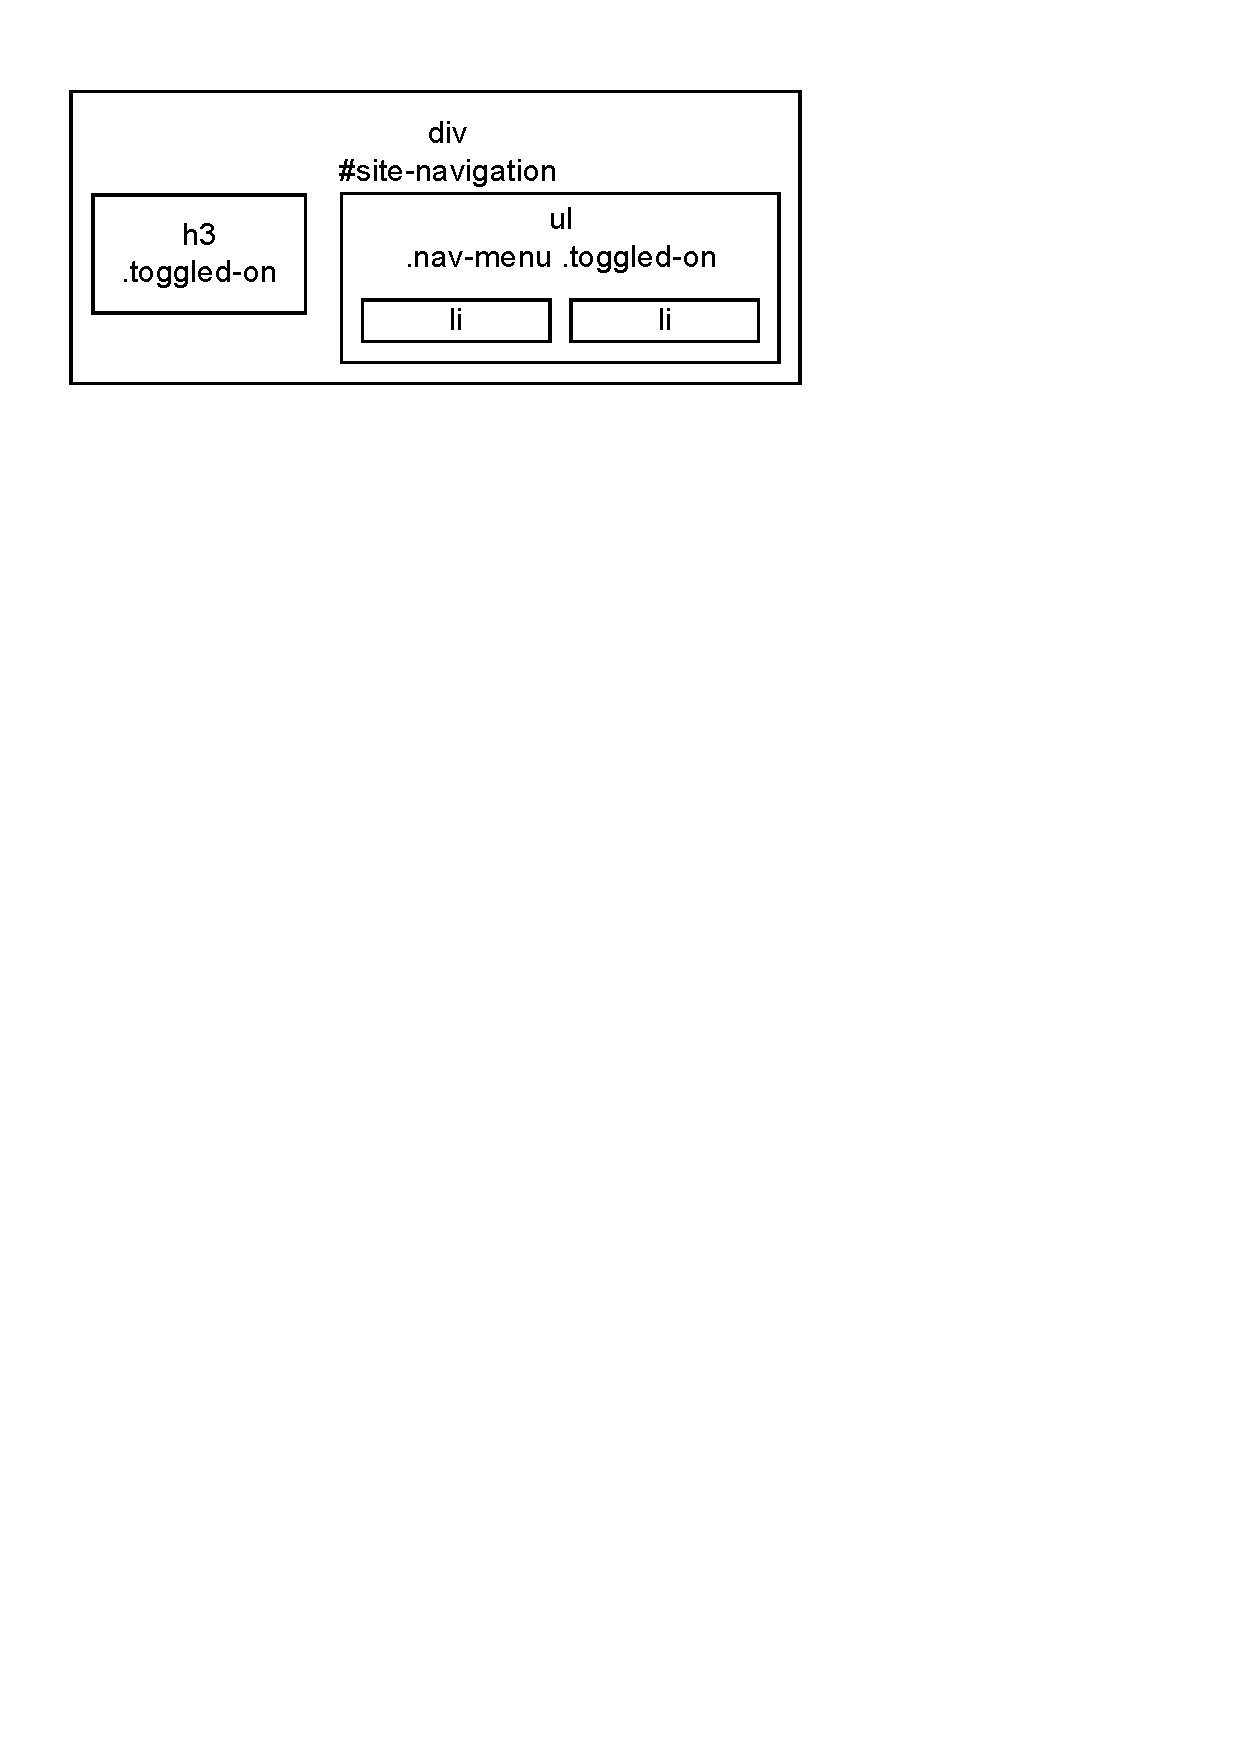
\includegraphics[width=55mm]{images/layout.pdf}
		\caption{Web page layout for the \javascript code}
		\label{Fig:Layout}
	\end{figure}
	
	The web application pertaining to \figref{Example} consists of a navigation menu with id \texttt{site-navigtion} at the top of the web page. The navigation menu contains one \texttt{h3} element and one \texttt{ul} element that contains some \texttt{li} elements that constitute the menu items. The menu is enabled when class \texttt{toggled-on} is added to the \texttt{h3} and \texttt{ul} elements and disabled otherwise. \figref{Layout} represents the layout of the subset of web page that the \javascript code in \figref{Example} is interacting with.
	
	The \javascript code first points references to various DOM elements (Line 7-10). The code then checks for the existence of certain DOM elements and returns if these elements are not present in DOM (Line 11-18). If the elements are present, the code then attaches an \texttt{onclick} event handler to the \texttt{h3} element (Line 20) which when clicked enables / disables the navigation menu by adding and removing the class \texttt{toggled-on} (Line 24 to 30). The code also makes sure that the class \texttt{nav-menu} is attached to the \texttt{ul} element (Line 21-22). The \javascript code assumes that the DOM structure of the web page always contains the element with id \texttt{site-navigation} where the existence of \texttt{h3} and \texttt{ul} elements is not mandatory within the element with id \texttt{site-navigation}.
	
	The \javascript code in \figref{Example} throws a null pointer error if navigation wrapper markup is removed from web page header.\footnote{\url{https://core.trac.wordpress.org/ticket/22307}} This error points to the fact that the programmer always assumed the presence of navigation menu in the web page and was not aware of the situation when this menu can be missing from the web page. To avoid this null pointer error a fix was suggested to exit the function if the navigation menu is not present on the web page. \figref{Fix} represents the suggested fix for the above mentioned error.
	
	We note that the error arises due to the lack of complete knowledge about the possible DOM states by the developer. To eliminate such errors the programmers need tools that can analyze possible DOM structures and provide suggestions to the developer. However, once different possible DOM states has been analyzed the fix for the above error is straight forward.
	
	
	\begin{figure}
	\medskip
	\begin{lstlisting}
	if ( ! nav )
		return;
	\end{lstlisting}
	\caption{Suggested fix}
	\label{Fig:Fix}
	\end{figure}
	
	
	
	\subsection{JavaScript Code Completion}
	\label{Sec:Code-completion}
	
	Although \javascript is syntactically similar to other languages such as Java, there are a number of differences that makes JavaScript different for providing code completion features.
	
	
	\headbf{Dynamically typed}
		In a dynamically typed language such as \javascript, every variable name is (unless it is null) bound only to an object. Names are bound to objects at execution time by means of assignment statements, and it is possible to bind a name to objects of different types during the execution of the program. Whereas, in case of statically typed language such as Java, every variable is bound both to a type as well as an object. Once a variable name has been bound to a type (that is, declared) it can be bound (via an assignment statement) only to objects of that type; it cannot ever be bound to an object of a different type. \figref{Typing} demonstrates the difference between strong and loose typing.

		\begin{figure}
			\begin{mdframed}
			\centering
			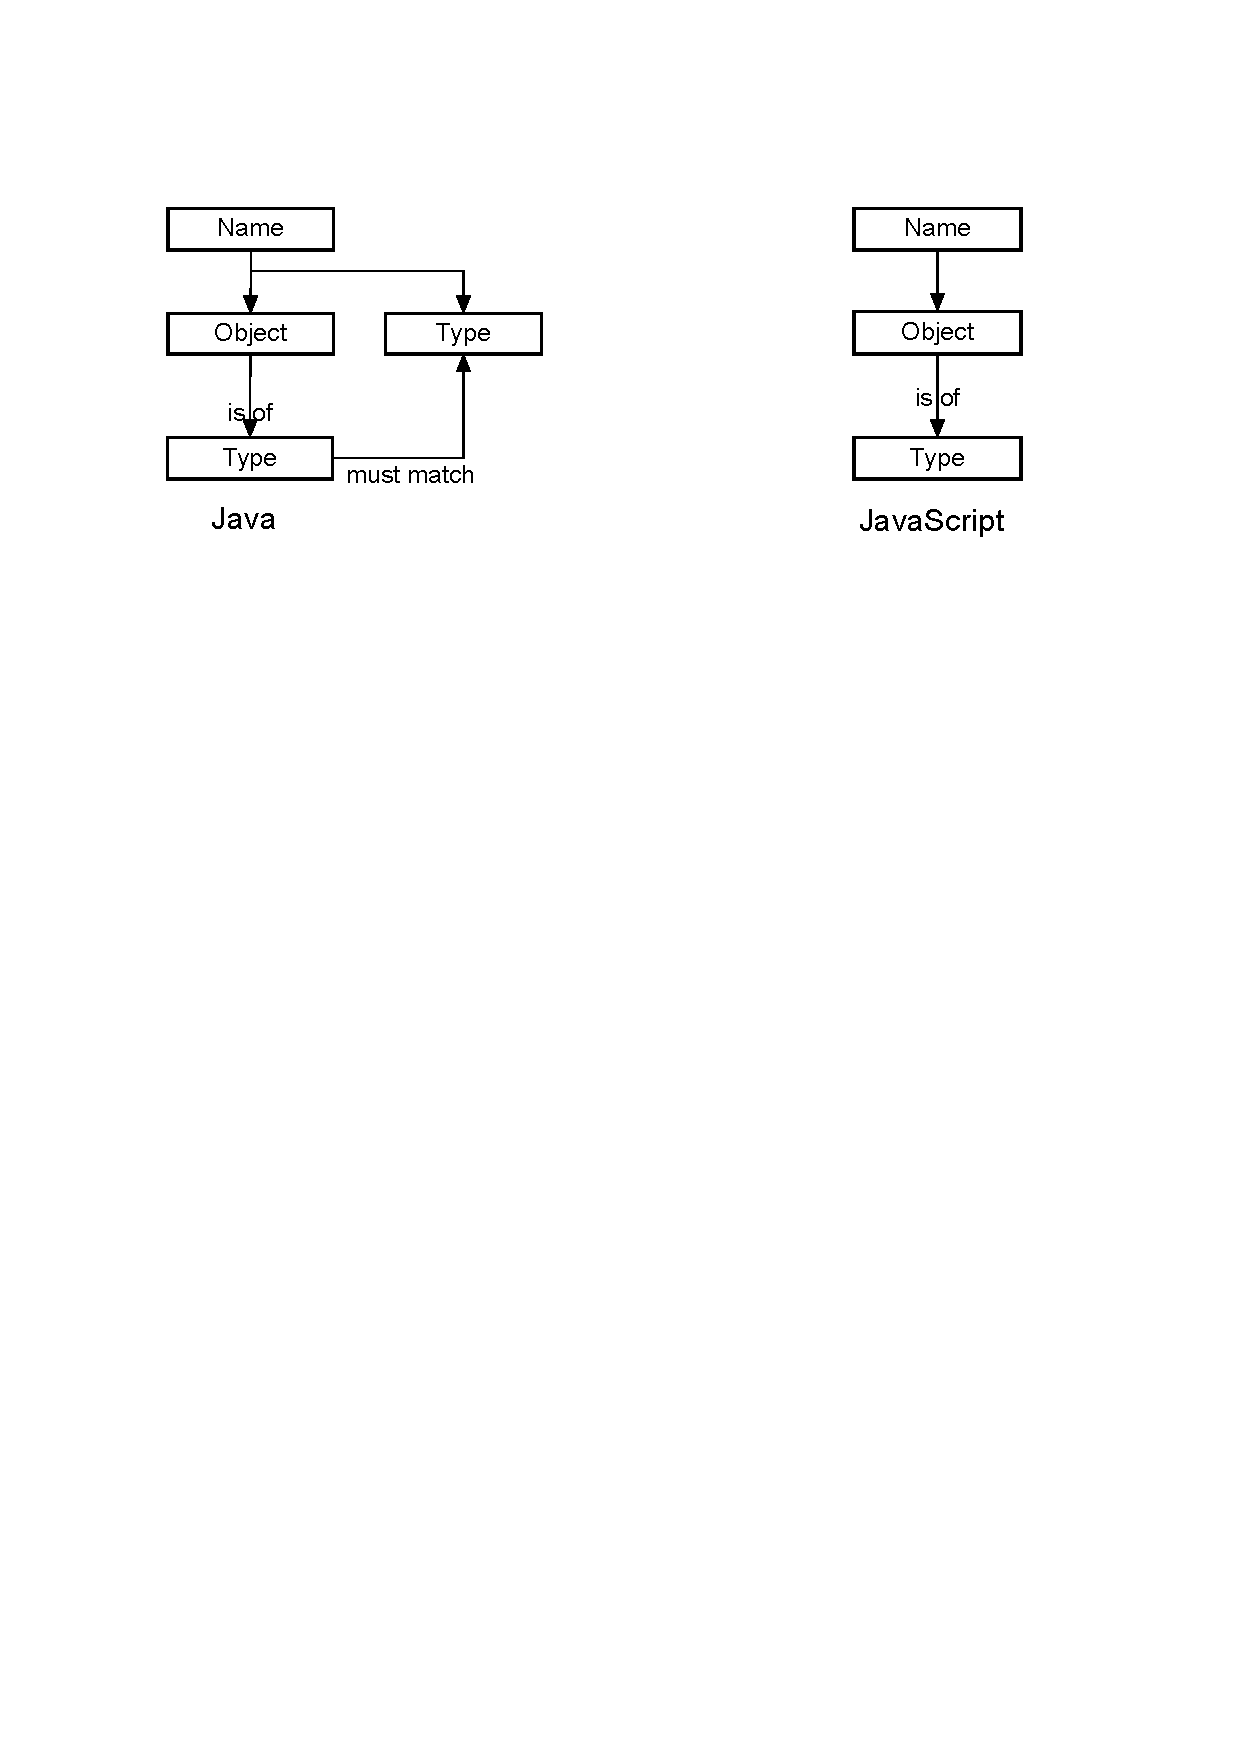
\includegraphics[width=75mm]{images/typing.pdf}
			\end{mdframed}
			\caption{Strong typing in Java vs. Dynamic typing in \javascript}
			\label{Fig:Typing}
		\end{figure}
		
		To provide features such as code completion we need to statically analyze the code and infer variable types. For strong typed languages a single pass through the code is enough to analyze variable types as variables are declared with fixed data type. Variables once attached to a particular type remain attached throughout the code execution. Therefore, developers can provide auto-complete features just by inferring the variable types by using simple static analysis of the code. Whereas, Dynamic typed feature of \javascript makes it difficult to analyze the variable types as these types can be modified during program execution \cite{hackett2012fast, kashyap2013type}. A variable attached to \texttt{int} type at the beginning of code execution might be attached to another type by the end of the code execution. 

	
	\headbf{DOM Interactions} \javascript code frequently interacts with DOM, \ie dynamic HTML generated within the web application. In the prior work~\cite{ocariza2013empirical} we have shown the prevalence of DOM related faults in the \javascript  code. \javascript uses DOM API calls, which in return points to the DOM elements. The DOM states can be manipulated using server side code(when the page loads) as well as client side code (after the page load). Therefore, when statically analyzing the \javascript code the value of variables can either be \texttt{null} if the target element is not present in DOM or it can be value returned from the DOM, therefore changing the type of \javascript variables without any change in the \javascript code. To effectively analyze the \javascript code, the knowledge about the DOM structure is required. 
	
	\subsection{Scope of the paper}
	\label{Sec:Scope}
	
	Prior work  has shown the prevalence of \javascript errors in the production websites.\cite{ocariza2011javascript} Further analysis revealed the presence of DOM related errors within \javascript code.\cite{ocariza2013empirical} There we choose to provide auto-complete suggestions for the DOM interactions within \javascript code. In this work we focus on 4 different methods within the DOM API that can be used to point references to the DOM elements.
	
	\begin{enumerate}
		
		\item \textbf{document.getElementById} 
		\item \textbf{document.querySelector} \\ \textbf{element.querySelector}
		\item \textbf{document.getElementsByClassName} \\ \textbf{element.getElementsByClassName}
		\item \textbf{document.getElementsByTagName} \\ \textbf{element.getElementsByTagName}
		
	\end{enumerate}
	
	\texttt{getElementById} function can only be called by the \texttt{document} object whereas the later 3 functions can also be called by any element within the DOM hierarchy, therefore making it possible to access any element within the DOM.
	
	
	
\section{Approach}
\label{Sec:Approach}

	Our DOM based Code-completion approach consists of 3 phases. 1) DOM analysis, 2) Code analysis, and 3) Suggestion generation. The \emph{DOM analysis} phase (\figref{DOM-Analysis}) involves crawling the web application and generate list of \css selectors present within the DOM states. The \emph{Code analysis} phase (\figref{Code-Analysis}) involves analyzing the \javascript code, creating list of in-scope variables and intercepting the DOM API calls that include reading and writing to the DOM. The results from the above two phases are passed to the \emph{suggestion generation} phase (\figref{Suggestions}) and combined to generate list of auto-complete suggestions that are presented to the developer. The DOM analysis phase is just executed once when the developer begins writing the code whereas Code analysis phases is executed every time when the developer tries to access the code-completion menu.
	
	\subsection{Usage Model}
	\label{Sec:Model}
		Because we focus on providing auto-complete for DOM based interactions, we assume that the developer has access to the web application under development. If the developer does not have access to the running web application, we assume that the developer has access to the HTML template of the website. Further, we assume that the JavaScript code within the editor is partially complete. By partially complete we refer to \javascript code that is syntactically correct and all the variables in use are defined and there are no global variables in use. The later assumption is based on the fact that usage of global variables within \javascript code is considered as a bad practice.\footnote{\url{http://stackoverflow.com/questions/10525582/why-are-global-variables-considered-bad-practice-javascript}}
		
		Our approach is designed to provide code completion suggestions for \javascript-DOM interactions within the \javascript code. There is no specific input required form the developer, other than hitting the code-completion menu while writing the code. DOM based code-completion is provided when any of the  functions mentioned in \tabref{API} are written by the developer.
	
	
		The output of our approach is a list of \css selectors which are shown as the developer is typing. The generated list is dependent on 1) \javascript variables in scope 2) Scope of parent element within DOM 3) Additions / deletions made to the DOM within the available code paths.
	
	\subsection{DOM Analysis}
	\label{Sec:DOM-Analysis}
		\begin{figure}
		%	\begin{mdframed}
			\centering
			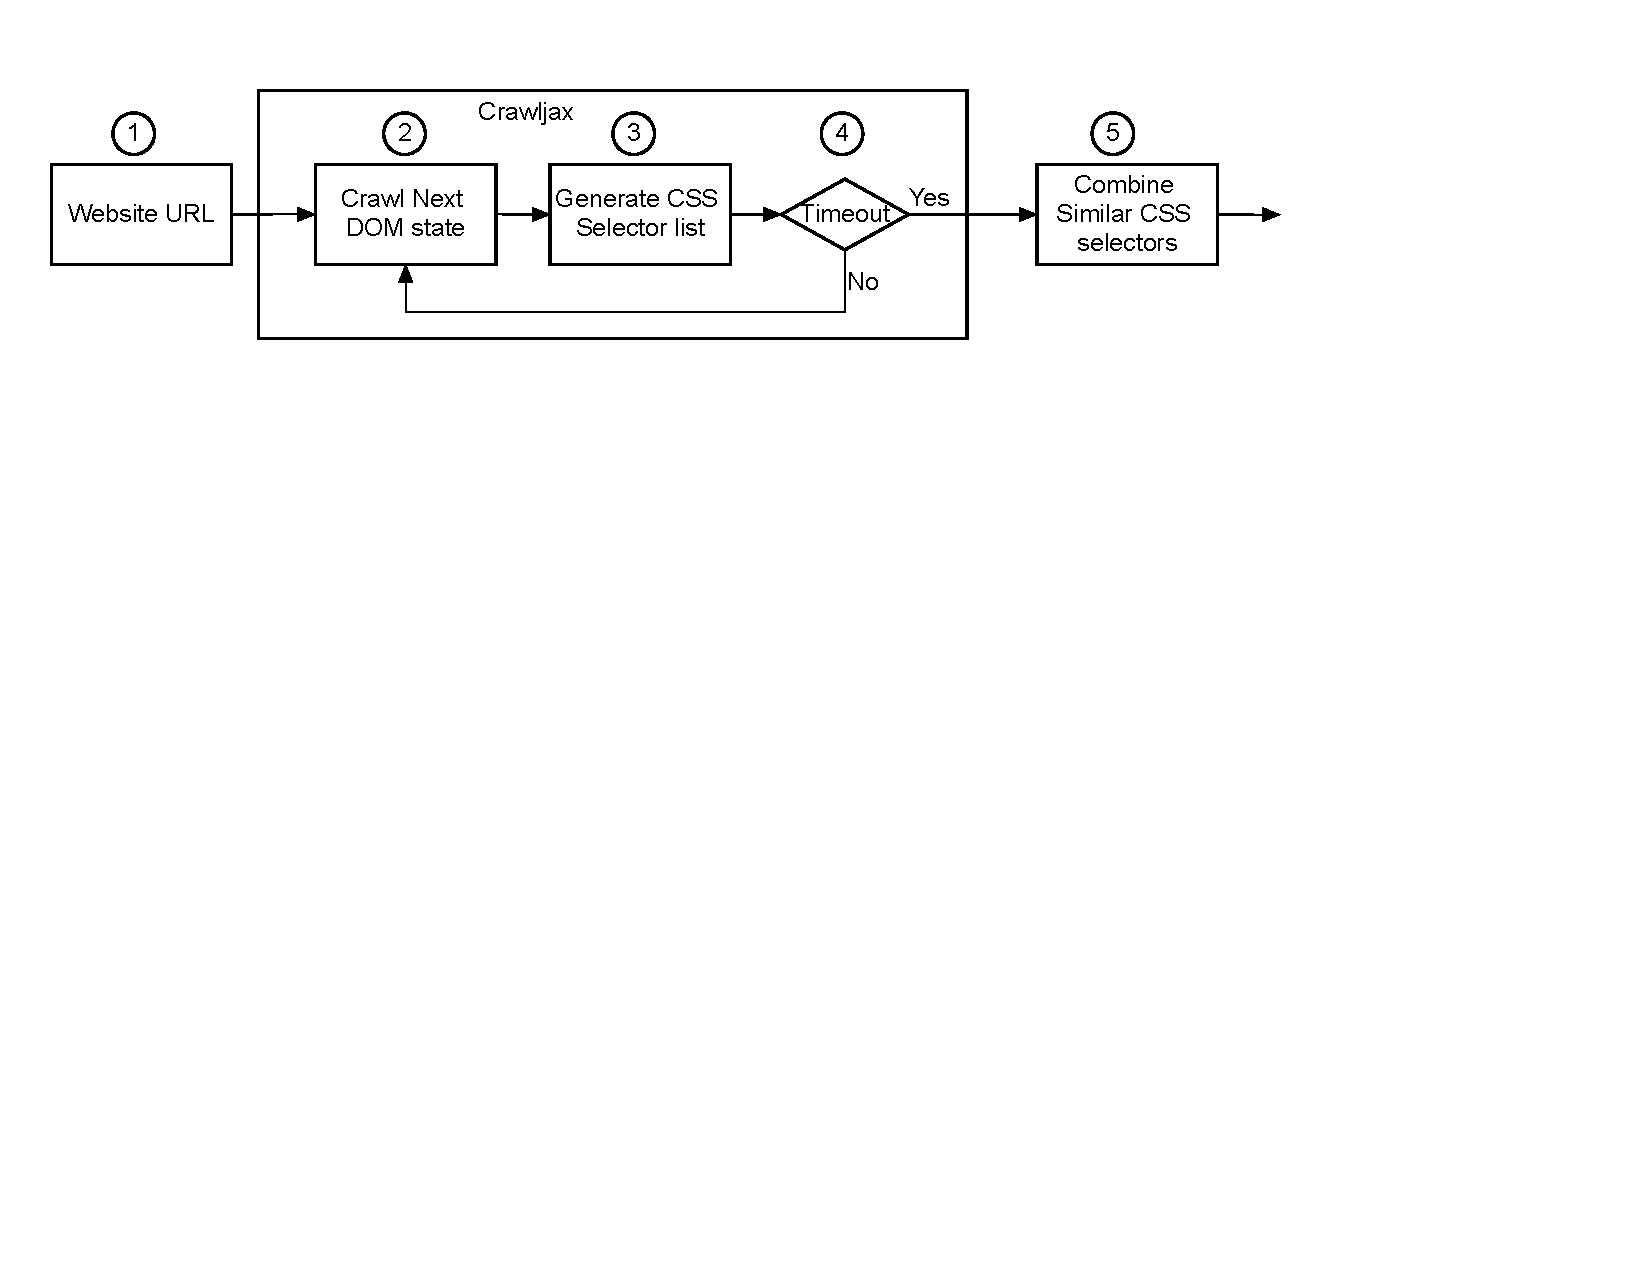
\includegraphics[width=85mm]{images/dom_analysis.pdf}
		%	\end{mdframed}
			\caption{DOM Analysis}
			\label{Fig:DOM-Analysis}
		\end{figure}
		In the DOM analysis phase, the corresponding web application is crawled (Step 2) using Crawljax \cite{crawljax:tweb12} to collect information about the DOM hierarchy and is then stored in the form of \css selectors\footnote{\css selectors are the patterns used to select particular DOM element} (Step 3). Each leaf node in the DOM is expressed as a sequence of tag name, id's and classnames found in the hierarchy. When one particular DOM state is stored in the form of \css selectors, the crawler moves to the next state. As the number of DOM states within the website can be infinite, a timeout limit is set by the user. The process is continued until the timeout limit is reached (Step 4). Once the timeout has reached, the \css selectors generated from different DOM states are combined (Step 5) to generate a superset of \css selectors which are then used in the later phase.
		
		\headbf{Converting DOM to \css Representation}
		Every element within the DOM hierarchy can be addressed as a space separated sequence of nodes beginning from the root node. Each node is a DOM element and can be represented as a combination of tag name, id and list of classes attached to the element. For example for \figref{Layout} the \texttt{li} elements can be represented as follows:
			
		\begin{quote}
			\texttt{div\#site-navigation ul.nav-menu.toggled-on li}
		\end{quote}
			
		To represent complete DOM tree in terms of \css selectors, we focus on all the leaf nodes within the tree, \ie the elements within DOM that does not have any child element. For every leaf node we generate a sequence of its \css selectors; therefore covering all the DOM elements present within the DOM tree. The list of \css selectors for each DOM state are then accumulated together to generate a superset of \css selector strings. The \css representation of the DOM tree for a single DOM state holds the following properties:
		\begin{itemize}
			 \item Each word represents a node in the DOM tree with a combination of tag name(required), class name(if present) and id(if present).
			 \item Each row starts with the root element and traverses to one of the leaf nodes i.e each row represents one path from root node to leaf nodes.
			\item Number of rows is equal to number of leaf nodes.
			 \item Number of words in each string represents the depth of particular path
		\end{itemize}
		
		As the number of crawled DOM states increases, the number of rows in the \css representation increases exponentially, therefore increasing the space and time complexity of the approach. To effectively provide code-completion suggestions within a decent time frame, we need to minimize the \css representation of the superset that is generated after the timeout is reached.
		
		\begin{description}
			\item[Removing duplicates]
			The two leaf nodes in the DOM tree that follow exact DOM hierarchy \ie they have exactly same \css representation, one of them is removed. For example in \figref{Example} the 2 \texttt{li} elements follows same DOM hierarchy therefore we can consider only one of them for the analysis.
		
			\item[Combining Similar IDs]
			Two rows within the \css based representation that follow the following criteria are the combined to form a single row. 

			\begin{itemize}
				\item The distance between the root node and the leaf node should be equal.
				\item Tag names should be exactly similar at each level of hierarchy.
				\item Classes attached to each tag should be exactly same.
			\end{itemize}

			For example:
			
			\begin{quote}
				\texttt{ul.nav-menu.toggled-on li\#item1}
	
				\texttt{ul.nav-menu.toggled-on li\#item2}
			\end{quote}

			In the above two sequences, distance between root node and leaf node for the both the sequences is 1, tag sequence for the sequences is \texttt{ul li}. Classes attached to each element are exactly same. To replace the above two sequences, we generate a new sequence that has exactly same length, tag sequence and classes attached to those tags. We then combine ids that differ in the original sequences and add all of these in the new sequence. The new sequence generated looks like the following sequence:

			\begin{quote}
				\texttt{ul.nav-menu.toggled-on li\#item1\#item2}
			\end{quote}

			\item[Combining Similar Classes]
			Two rows within the \css based representation that follow the following criteria are the combined to form a single row. 
			
			\begin{itemize}
				\item The distance between the root node and the leaf node should be equal.
				\item Tag names should be exactly similar at each level of hierarchy.
				\item IDs attached to each tag should be exactly same.
			\end{itemize}

			For example:
			\begin{quote}
				\texttt{ul\#nav-menu.toggled-on li.item1}
	
				\texttt{ul\#nav-menu.toggled-on li.item2}
			\end{quote}

			In the above two sequences, distance between root node and leaf node for the both the sequences is 1, tag sequence for the sequences is \texttt{ul li}. Ids attached to each element are exactly same. With the approach similar to the previous case the new sequence is generated.

			\begin{quote}
				\texttt{ul\#nav-menu.toggled-on li.item1.item2}
			\end{quote}
			
			The resulting \css representations might not result in valid \css selectors (such as having two IDs together is invalid). However, we are using this information for code-completion purpose and not for selecting DOM elements.
		
		\end{description}
	
	\subsection{Code Analysis}
	\label{Sec:Code-Analysis}
		\begin{figure}
		%	\begin{mdframed}
			\centering
			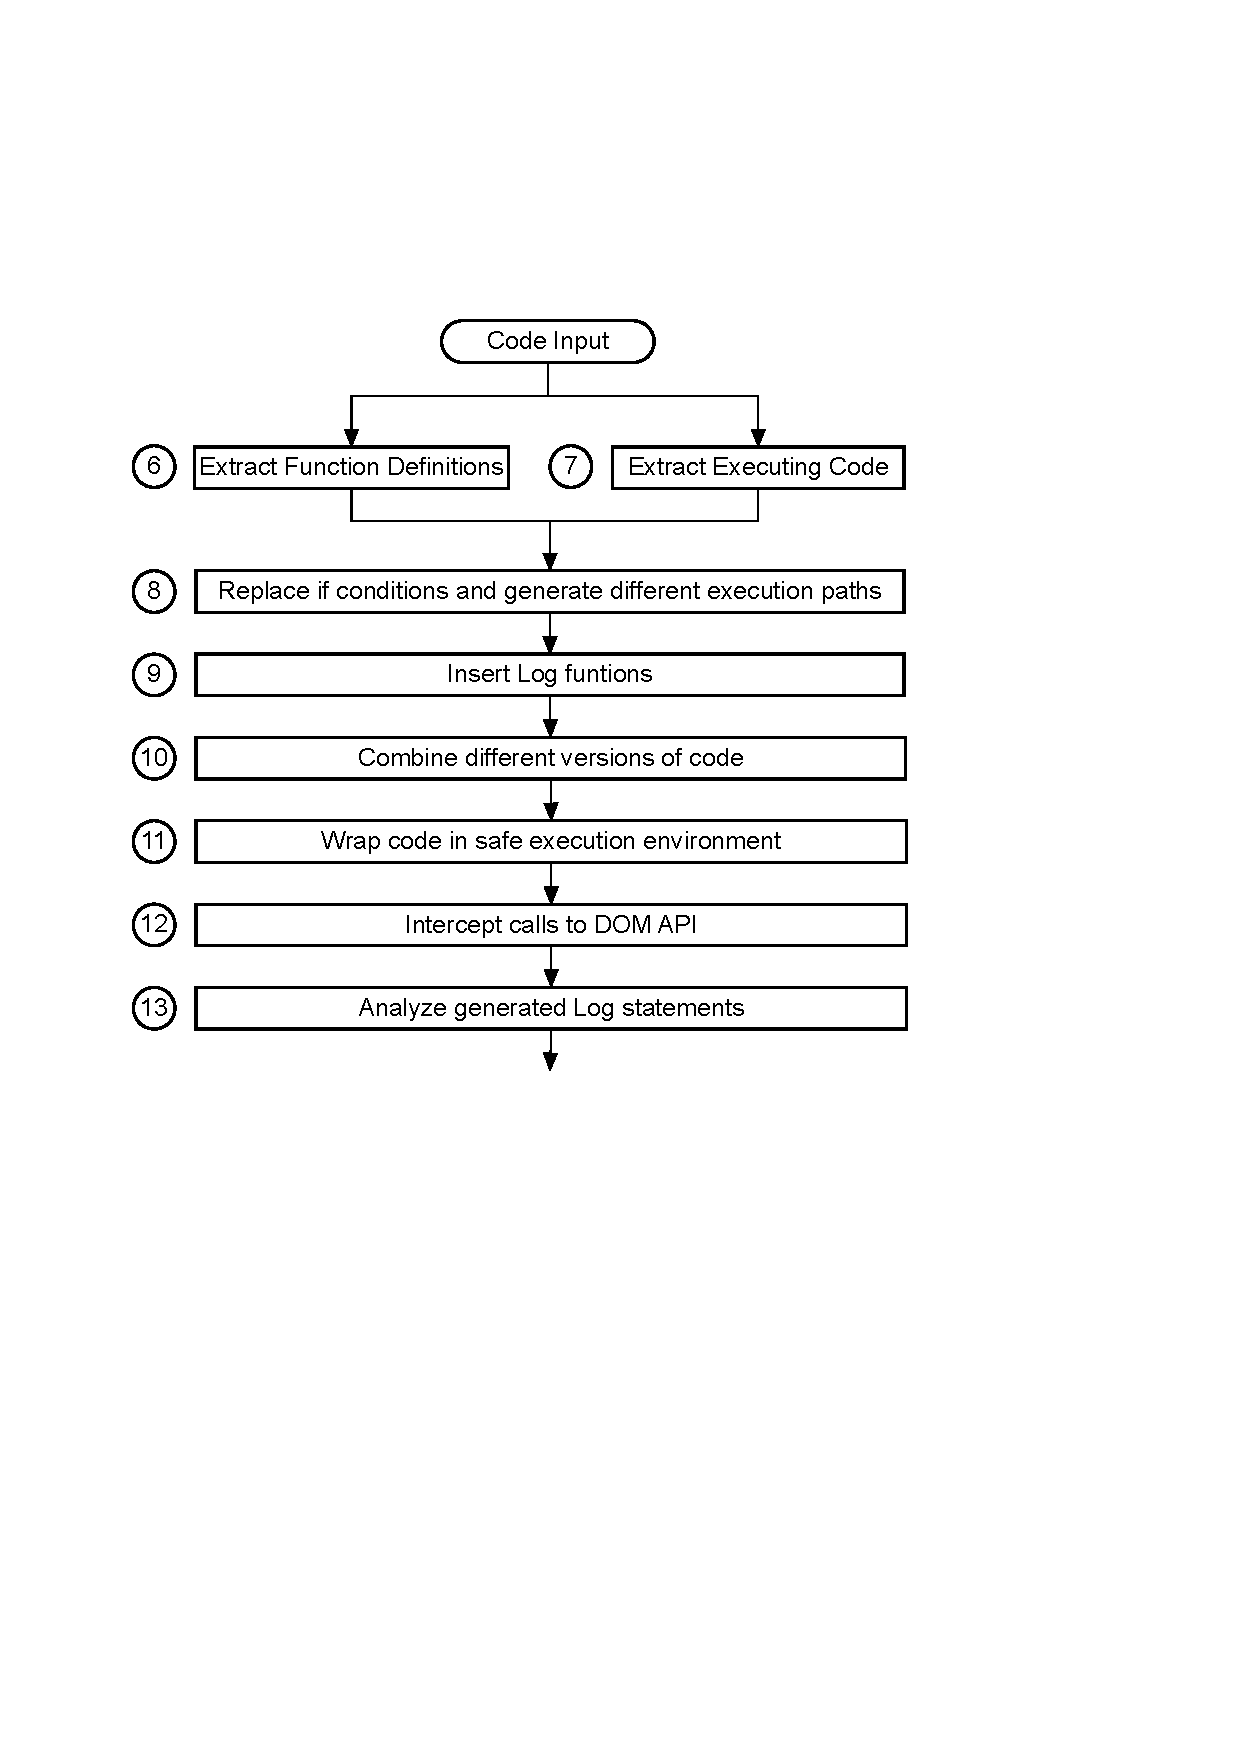
\includegraphics[width=85mm]{images/code_analysis.pdf}
		%	\end{mdframed}
			\caption{Code Analysis}
			\label{Fig:Code-Analysis}
		\end{figure}
		
		In the Code Analysis phase, the \javascript code available within the editor is parsed to extract function definitions (Step 6) and the executing code segment (Step 7). Both the function definition and the executing code segment are then modified to replace the \texttt{if} conditions (Step 8) generating a maximum of $2^n$ different versions, where $n$ is the number of \texttt{if} conditions within that code segments. For each newly generated code path, relevant log statements are inserted within the code to keep track of the code path (Step 9). Based on the executing code segment, calls are made to each version of function definition therefore covering all the possible code paths (Step 10). This execution of \javascript code is performed in a secure environment (Step 11) with dummy functions being returned for calls to \texttt{document} or \texttt{window} objects, as well as it intercepts these calls (Step 12) for analysis purpose. The logs generated after the code execution are then analyzed (Step 13) and a list of DOM elements referred in the code is generated. The results of this analysis are used as an input for the next phase.
		
		The entire execution of the code is wrapped in \texttt{try-catch} block to avoid any run-time error. It is highly likely to have syntax errors in the under development code. Such errors when encountered are reported to the user for the purpose of correction. Therefore, our approach also catches a large number of errors in the beginning stage only.
		
		
		\begin{figure}
			\medskip
			\begin{lstlisting}
	( function() {
		var nav = document.getElementById( 'site-navigation' ), button, menu;
		button = nav.getElementsByTagName( 'h3' )[0];
		menu   = nav.getElementsByTagName( 'ul' )[0];
		! button;
		dompleteLog("func1 T","");
		return;
		// Hide button if menu is missing or empty.
		if ( ! menu || ! menu.childNodes.length ) {
			button.style.display = 'none';
			return;
		}
		button.onclick = function() {
			if ( -1 == menu.className.indexOf( 'nav-menu' ) )
				menu.className = 'nav-menu';

			if ( -1 != button.className.indexOf( 'toggled-on' ) ) {	
				button.className = button.className.replace( ' toggled-on', '' );
				menu.className = menu.className.replace( ' toggled-on', '' );
			} else {
				button.className += ' toggled-on';
				menu.className += ' toggled-on';
			}
		};
	} )();
			\end{lstlisting}
			\caption{One possible code path within the executing code}
			\label{Fig:Path}
			\end{figure}
			
			
			\begin{figure}
			\medskip
			\begin{lstlisting}
	create #site-navigation, 
	local nav|#site-navigation, 
	create #site-navigation h3, 
	local button|#site-navigation h3, 
	create #site-navigation ul, 
	local menu|#site-navigation ul, 
	func1 T 
			\end{lstlisting}
			\caption{Logs generated after path execution}
			\label{Fig:Logs}
			\end{figure}
			
		
		\headbf{Replacing \texttt{if} conditions}
		When writing code, different actions are performed based on different decisions. Conditional statements like \texttt{if else} are used in the code to indicate these decisions. Each decision creates a new branch within the code therefore increasing the possible number of code paths that can be followed within the code. To provide auto-complete feature, we need to analyze every possible path within the available \javascript code.
		
		These conditions are removed recursively from the code, where each recursion results in 2 different versions of the code and then recursively performing the same task on the new versions. The process is continued until all the conditions are removed from the code. The conditional statement within the \texttt{if} condition will always be executed irrespective of what path does the code takes at that point. In addition to this, log statements are inserted to keep track of the code path followed within that version of code. Loop statement such as \texttt{for} and \texttt{while} could also reflect the possible code paths. However in our implementation, if the loop condition is dependent on the DOM, the code within the loop will be executed at least once. Otherwise number of loops will be dependent on the value of variables within the code. We discuss more about loops in the \secref{Limitations}
		
		For the example given in \figref{Example}, when the developer is trying to access the code-completion functionality while adding new code in the end, there is one function defined from Line 6-32, with the call to the defined function at Line 32. The executing code segment would be Line 32 followed by the code execution in the function. A total of 16 different code paths are generated and the results for the code-completion will reflect all these paths. \figref{Path} represents one possible code path. The first \texttt{if} condition is removed from the code and the code path with \texttt{true} block is executed. Note that the code after Line 7 will not be executed due to the execution of \texttt{return} statement. The logs generated after executing this code path are presented in \figref{Logs}.	
		
		
				
			\begin{figure}
			\medskip
			\begin{lstlisting}
	if(document.getElementById != undefined) { 
		document._oldGetElementById = document.getElementById; 
			
		document.getElementById = function(id) { 
			var result = document._oldGetElementById(id); 
				
			if (!result) { 
				addInnerHTML(document,"<div id=\'" + id + "\'></div>"); 
				result = document._oldGetElementById(id); 
				result = createProxy(result,document.csspath + " #" + id); 
			} 
			result.appended = true;
			result = createProxy(result,document.csspath + " #" + id);
			dompleteLog("create " + result.csspath,"");
			return result; 
		}; 
	}
			\end{lstlisting}
			\caption{Intercepting calls to \texttt{getElementById} function}
			\label{Fig:Environment}
			\end{figure}
			
		
		\headbf{Execution Environment}
			\javascript code contains references to global objects available within the browser. These objects can be classified into two main categories: 1) Browser Objects and 2) HTML DOM Objects. Browser objects include window\footnote{\url{http://www.w3schools.com/jsref/obj_window.asp}}, navigator\footnote{\url{http://www.w3schools.com/jsref/obj_navigator.asp}}, screen\footnote{\url{http://www.w3schools.com/jsref/obj_screen.asp}}, history\footnote{\url{http://www.w3schools.com/jsref/obj_history.asp}},  and location\footnote{\url{http://www.w3schools.com/jsref/obj_location.asp}}. HTML DOM objects include document\footnote{\url{http://www.w3schools.com/jsref/dom_obj_document.asp}}, and element\footnote{\url{http://www.w3schools.com/jsref/dom_obj_all.asp}} objects. These objects expose an API that can be used to interact with the browser and the HTML within it. Faulty interactions with these APIs can lead to an unexpected output. Therefore to securely execute the code we need to create a safe execution environment that can prevent these interactions from causing a fault.
			
			To securely execute the \javascript code, we redefine functions within these objects and dummy objects are returned based on the return type of the function. We also insert log statements to keep track about when the particular function was called and what were the parameters passed to it. Additional variables are added for the code analysis purpose. Every reference to DOM element returned by these re-defined functions contains a property named \texttt{csspath} to keep track of the \css selectors attached to that element. \figref{Environment} provides an example where a call to \texttt{getElementById()} function is being intercepted.

	
	\subsection{Suggestion Generation}
	\label{Sec:Suggestions}
		\begin{figure}
		%	\begin{mdframed}
			\centering
			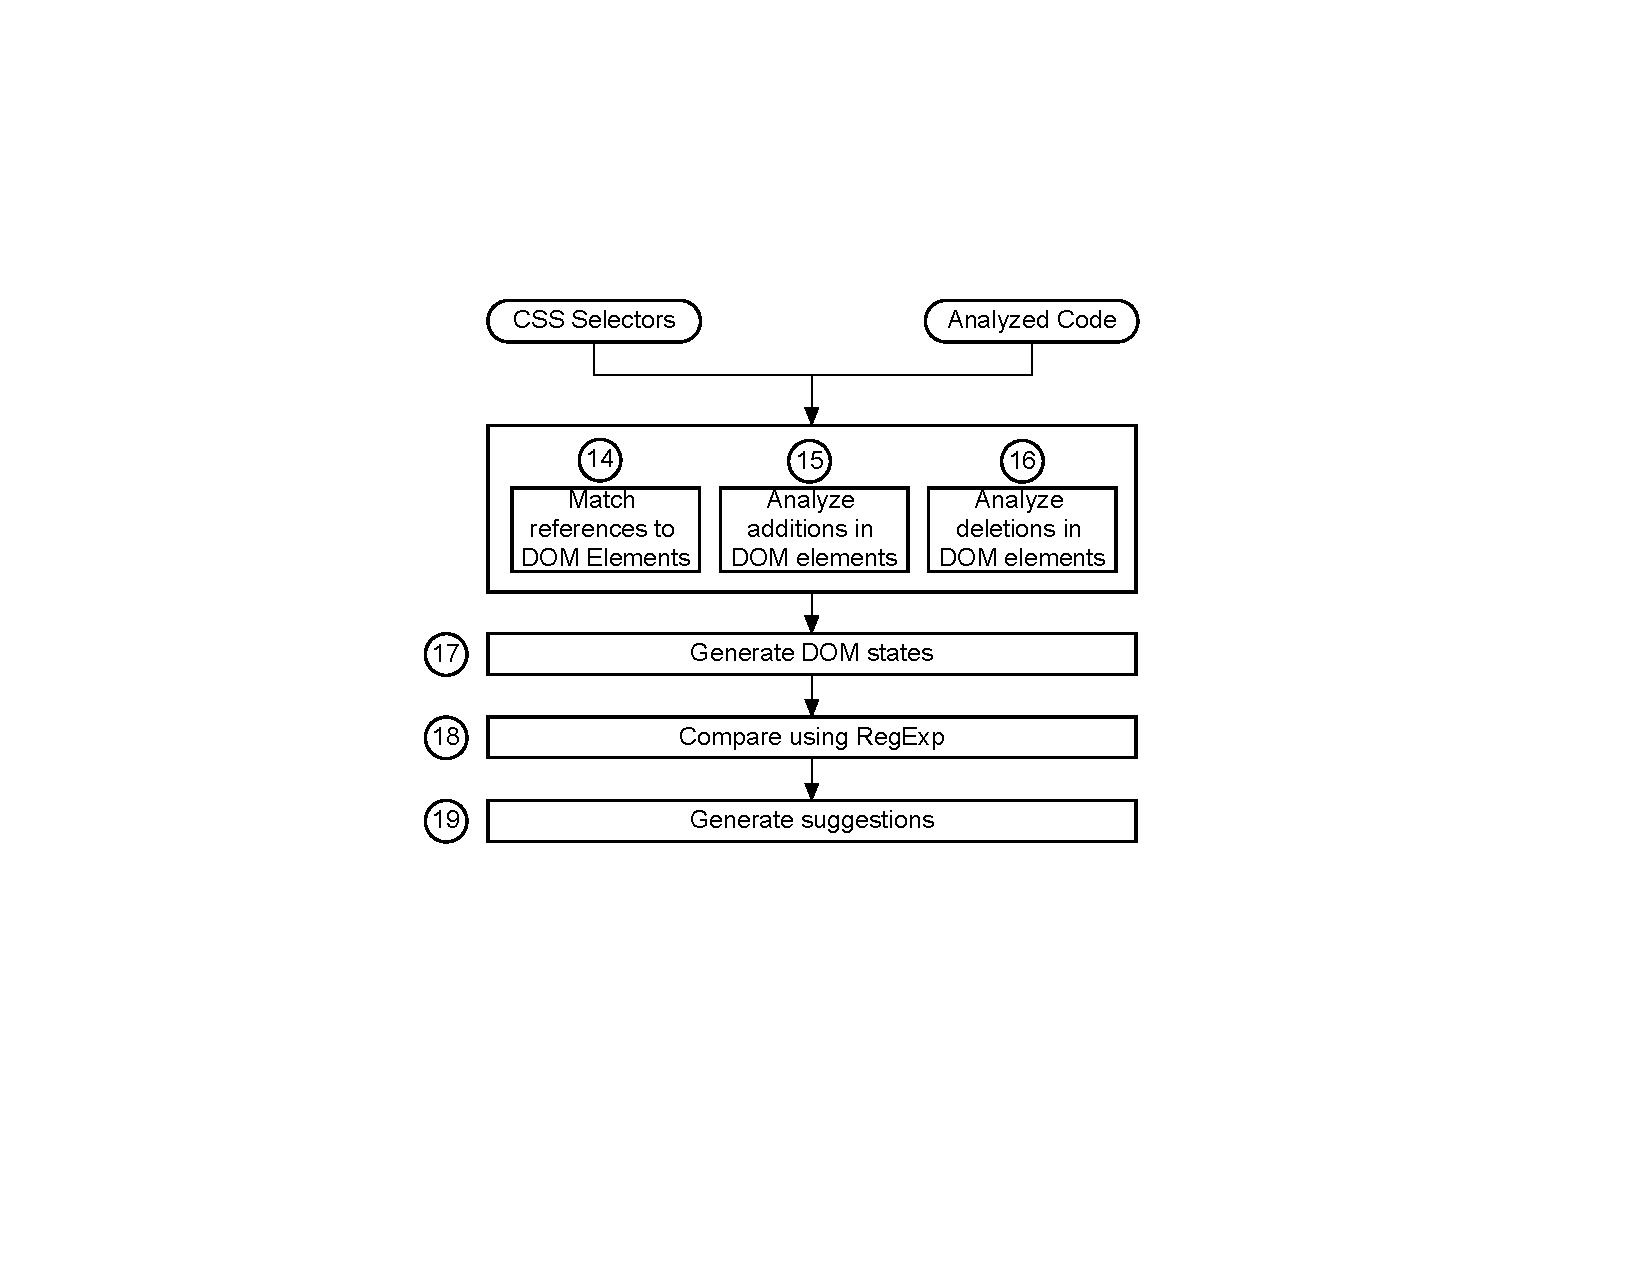
\includegraphics[width=85mm]{images/suggestions.pdf}
		%	\end{mdframed}
			\caption{Suggestion Generation}
			\label{Fig:Suggestions}
		\end{figure}
		
		The outputs from the DOM analysis and Code analysis phase are used as an input to the Suggestion generation phase. The references to DOM generated in code analysis phase are matched against the CSS selectors generated in the DOM analysis phase. Anomalies with respect to DOM elements are then highlighted and presented to the user (Step 14). Possible effects of DOM modifications (Step 15-16) within the \javascript code are also analyzed. The results of the analysis are used to generate the possible DOM states (Step 17). These DOM states in combination with the input specified in the \secref{Model} are matched using regular expressions (Step 18) to provide code-completion suggestions to the user (Step 19). The suggestions presented to the user reflect the scope of parent element within the new DOM.
		
					\begin{figure}
			\medskip
			\begin{lstlisting}
		re1 = /[^#\\. ]*(?=[ \\.#])#site-navigation(\\.[^\\.# ]+)*(\\([^\\)]+\\))*(?=[ ])/;
			
		re2 = /h3(#[^#\\. ]+)*(?=[ \\.])(\\.[^\\.# ]+)*(\\([^\\)]+\\))*(?=[ ])/;
			\end{lstlisting}
			\caption{First regular expression matches any type of DOM element with \texttt{id=`site-navigation'} and any number of classes attached to it. Second regular expression matches all the \texttt{h3} tags with any id and any number of classes attached to them, within the child elements of the previously matched element.}
			\label{Fig:RegExp}
			\end{figure}
		\headbf{Creating Regular Expressions for matching}
			All the DOM variables within the \javascript code have an additional property \texttt{csspath} (refer to previous section) attached to them. A regular expression is generated to match the superset of DOM elements within the generated DOM that contains the sequence of \css selectors mentioned in the \texttt{csspath} variable. These DOM elements act as a possible parent for the current code-completion context. All the child elements for these parent elements are then combined to generate code-completion suggestions. \figref{RegExp} represents regular expressions for the value of \texttt{button.csspath} variable \ie \texttt{`\#site-navigation h3'} at Line 9 in \figref{Example}.
		
		
\section{Implementation}
\label{Sec:Implementation}

We have implemented the approach described in \secref{Code-Analysis} in a tool called Dompletion using \javascript programming language. This tool is built on top of the existing online code editor ACE~\footnote{\url{http://ace.c9.io/}}.


\section{Evaluation}
\label{Sec:Evaluation}

	\subsection{Goals and Research Questions}
	\label{Sec:Goals}
	In order to evaluate how effective is our tool in assisting the developers, we empirically evaluated our tool as well as conducted an a user study. We wish to answer the following research questions in our study.
	\begin{description}
		\item[RQ1:] What is the convergence rate for number of unique CSS selectors verses number of DOM states?
		\item[RQ2:] How accurate are the code-completion suggestions provided by the tool?
		\item[RQ3:] How is the list of code-completion suggestions affected by each phase of our analysis?
		\item[RQ4:] Does \dompletion make programming tasks faster without compromising correctness of the program?
		\item[RQ5:] Does \dompletion make debugging tasks easier?
%		\item[RQ5:] What is the overhead
		
	\end{description}
	
	\subsection{Methodology}
	\label{Sec:Methodology}
	The subsection that follow address each of the above questions. An overview of the evaluation methodology we have used to answer each research questions is shown below.
	
	\headbf{RQ1 Approach} We answer this question by conducting a study on 5 major websites including a few listed in top 100 websites on Alexa\footnote{\url{http://www.alexa.com/topsites}}. We crawl these websites in a random order until the number of unique css selectors become constant.  We then report the number of DOM states crawled for each website.
	
	\headbf{RQ2: Approach} To answer this question, we use our tool to generate suggestions for an existing php-\javascript based web application. We then manually match the list of generated suggestions to the existing text within the \javascript code. The list of generated suggestions is considered valid if one of the suggestions matches the \css selector used within the code where the code completion was initiated.
	
	\headbf{RQ3: Approach} To answer this question, we modified our tool to include / exclude different analysis phase, therefore affecting the length of suggestions generated by the tool. We then report the effect of each phase on the results.
	 	
		\begin{figure}
		\centering
		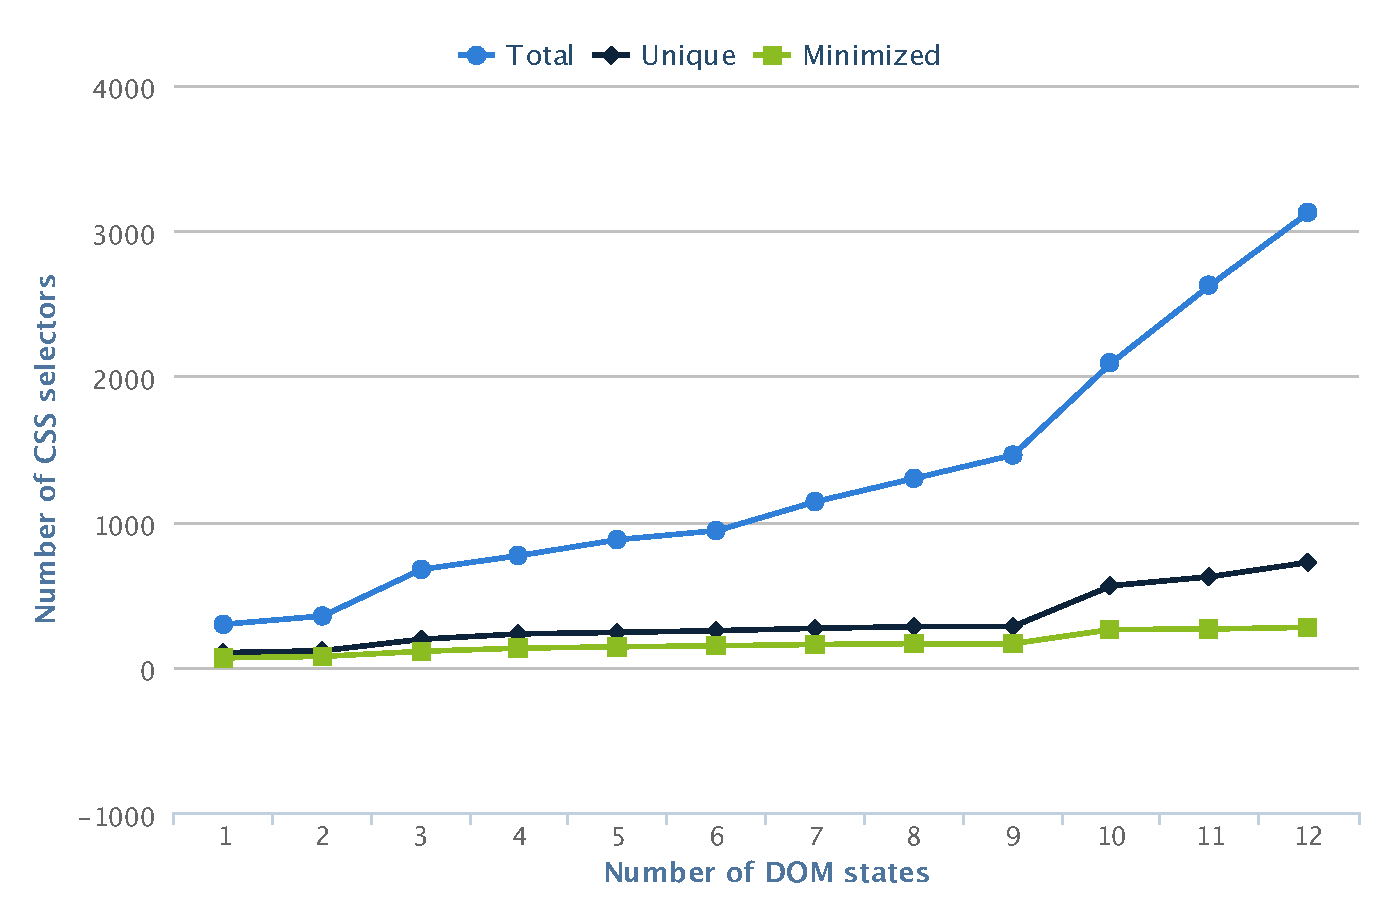
\includegraphics[width=85mm]{images/facebook.pdf}
		\caption{CSS Selectors for user dependent content (Facebook)}
		\label{Fig:Facebook}
	\end{figure}
	\begin{figure}
		\centering
		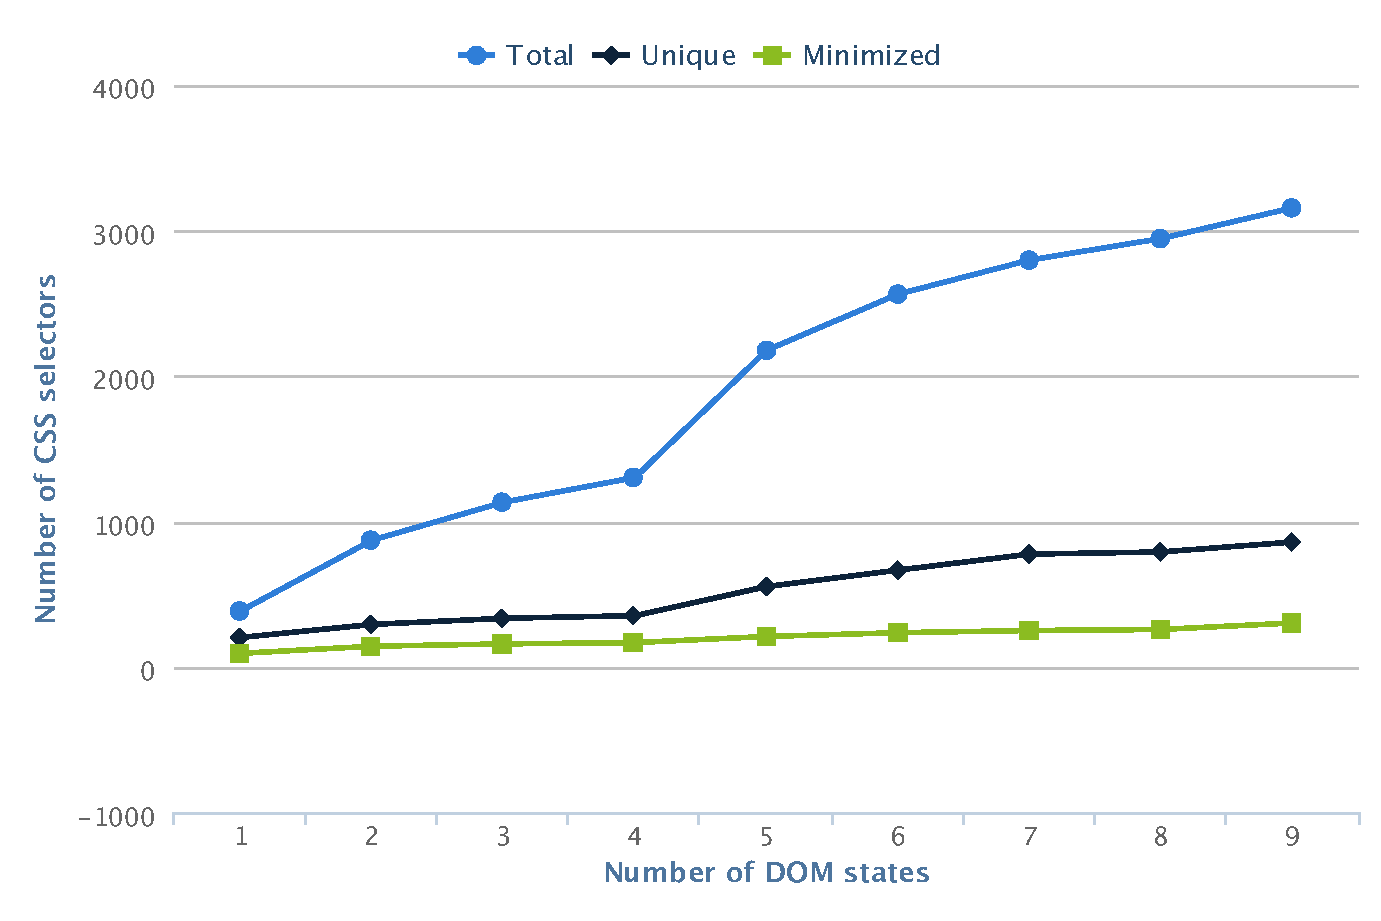
\includegraphics[width=85mm]{images/wikipedia.pdf}
		\caption{CSS Selectors for user generated content (Wikipedia)}
		\label{Fig:Wikipedia}
	\end{figure}
	\begin{figure}
		\centering
		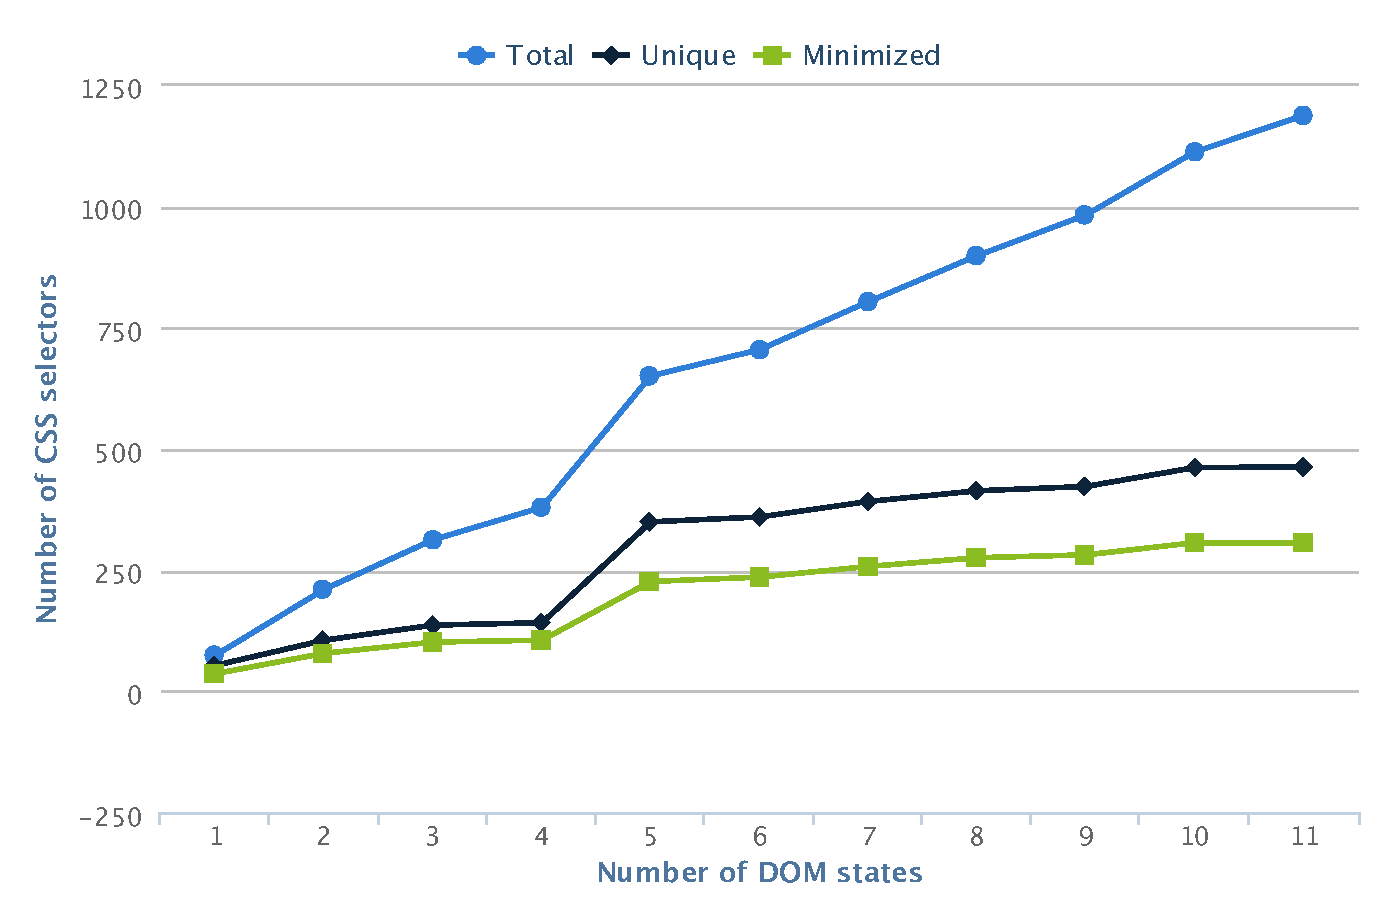
\includegraphics[width=85mm]{images/bing.pdf}
		\caption{CSS Selectors for Search Engine (Bing)}
		\label{Fig:Bing}
	\end{figure}
	\begin{figure}
		\centering
		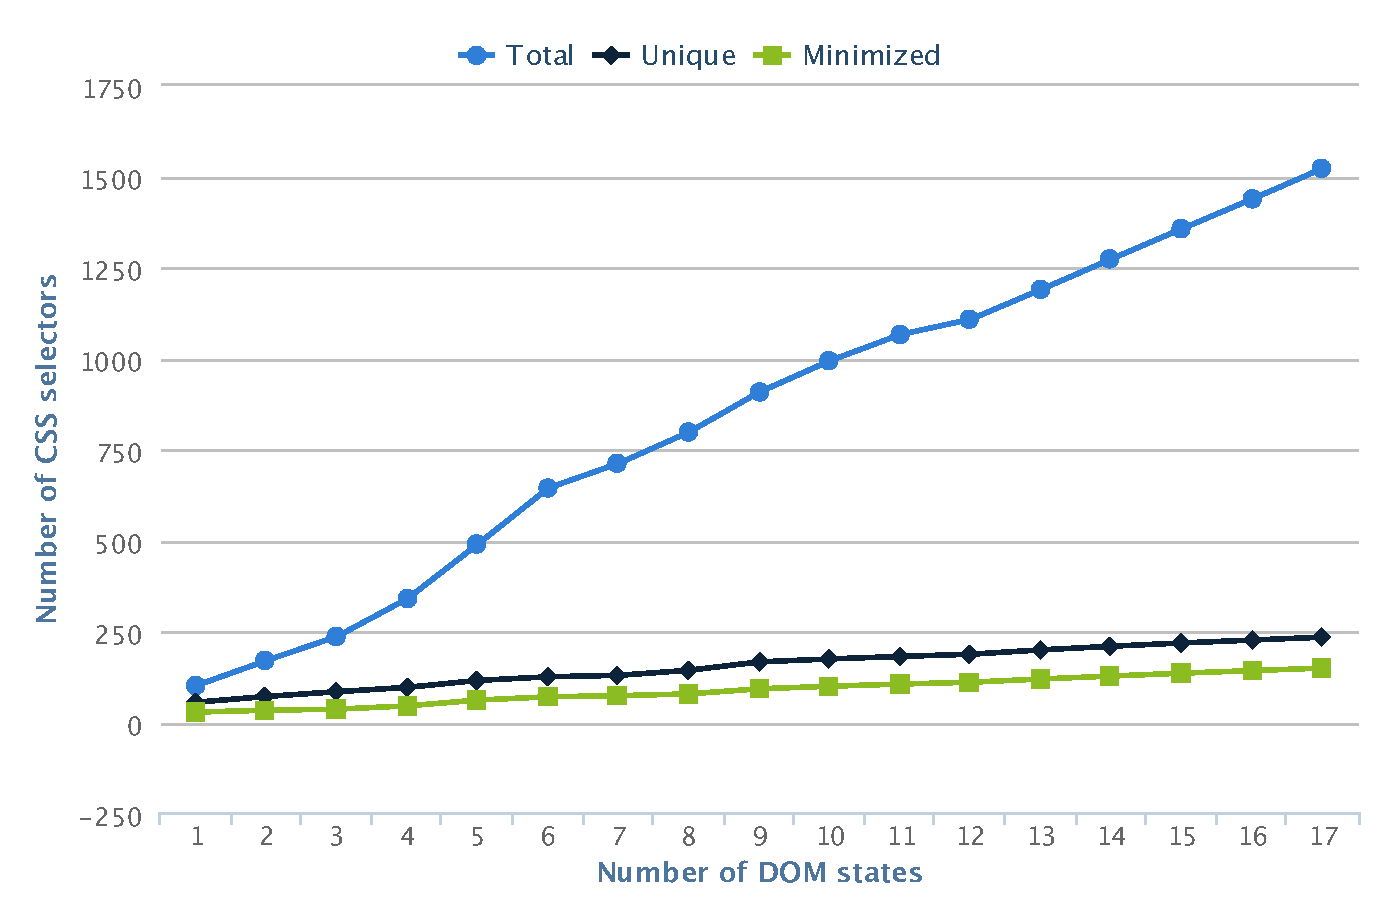
\includegraphics[width=85mm]{images/wordpress.pdf}
		\caption{CSS Selectors for blog (Wordpress)}
		\label{Fig:Wordpress}
	\end{figure}
	\begin{figure}
		\centering
		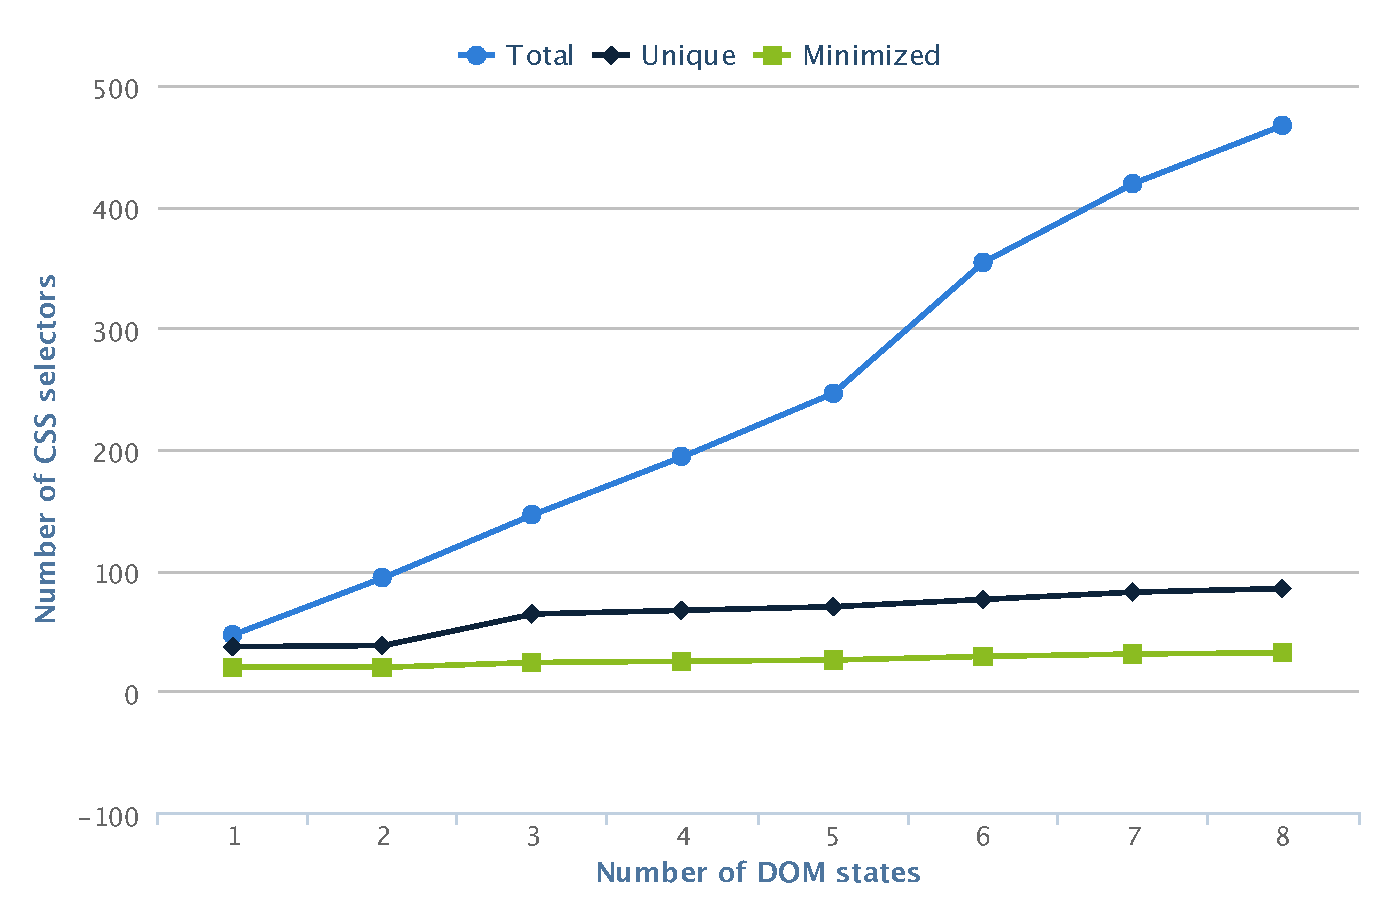
\includegraphics[width=85mm]{images/ajax.pdf}
		\caption{CSS Selectors for AJAX based website (Blog)}
		\label{Fig:AJAX}
	\end{figure}
	
	\subsection{Convergence rate for \css selectors}
	\label{Sec:Convergence}
	To answer RQ1, we crawled 5 web applications: Facebook\footnote{\url{https://www.facebook.com/}} (User specific content), Wikipedia\footnote{\url{https://www.wikipedia.org/}} (User generated content), Bing\footnote{\url{http://www.bing.com/}} (Search Engine), Wordpress Blog\footnote{\url{http://blogs.ubc.ca/karthik/}} and AJAX based blog\footnote{\url{http://www.ece.ubc.ca/~amesbah/}}. All the applications chosen for analysis were dynamic in nature, \ie the DOM tree generated for these websites is either user or input dependent. We also analyzed two blogs where content of DOM tree is dependent on one single user (blog admin) and similar for other user. 
	
	For each web application, we started crawling their home page. We counted the total number of \css selectors, total number of unique \css selectors and total number of minimized \css selectors. For every successive DOM states we included the list of \css selectors from the previous states, therefore only measuring the new \css selectors encountered at each state. 
	
	\figref{Facebook} - \ref{Fig:AJAX} represent the results of analysis at the  end of each DOM state for different websites. As seen from the results, all of the above mentioned websites exhibit patterns in their \css selectors and these patterns tend to converge quickly. The patterns once detected can be used to predict the structure of DOM states that were not encountered during the crawling phase. Therefore, the code-completion system can detect patterns and provide suggestions even for the unseen but similar DOM states.
	
	\finding{DOM states for a particular website exhibit patters in their \css selectors and these patterns tend to converge with increasing number of DOM states. \label{Finding:Convergence}}
	
	
	\begin{figure}
		\centering
		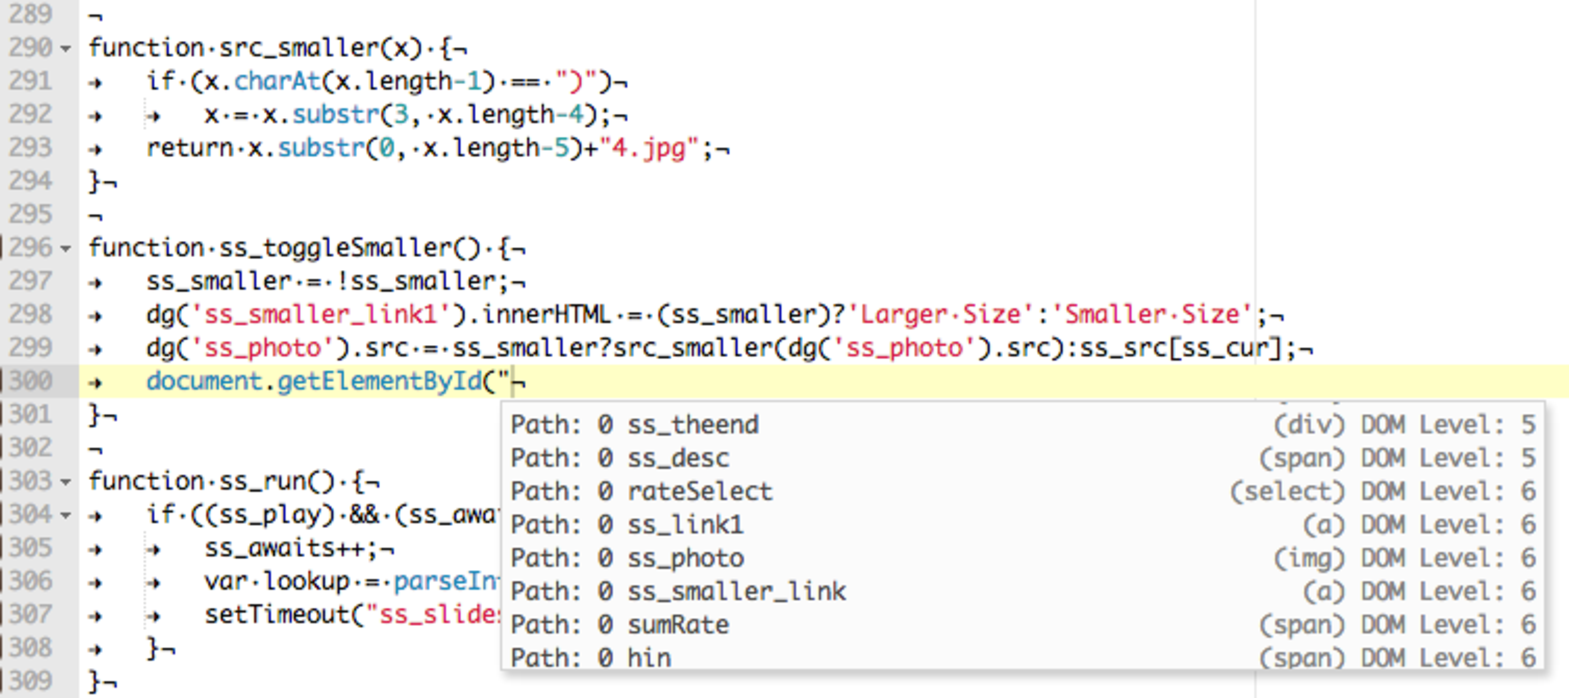
\includegraphics[width=85mm]{images/accuracy.pdf}
		\caption{Code completion suggestions generated using \dompletion}
		\label{Fig:Accuracy}
	\end{figure}
	
	\begin{table}
	{
		\scriptsize
		\begin{tabular}{ p{3.8cm} | p{3.8cm}}
  			\hline                        
  			\textbf{Output} & \textbf{No. of use cases} \\ \hline \hline
  			Valid Suggestions &  40 \\ \hline
			Invalid Suggestions & 7 \\ \hline
			Error & 6 \\ \hline
			Total & 53 \\ 
			\hline  
		\end{tabular}
	}
	\caption {\dompletion evaluation}
	\label{Table:Accuracy}		
	\end{table}
	
	
	
	
	\subsection{Accuracy of \dompletion}
	\label{Sec:Accuracy}
	To answer RQ2, we performed our analysis using an existing php-\javascript based web application Phormer\footnote{\url{http://p.horm.org/er/}}. The choice of web application was based on the following factors:
	\begin{itemize}
		\item \textbf{No use of \javascript libraries:} As our tool \dompletion is in the beginning phase of development, we do not support \javascript libraries. Therefore we prefer to use a web application that does not use libraries. Also we first need to evaluate out tool using native \javascript functions followed by the extension to support \javascript libraries. We discuss about this in detail in \secref{Discussion}.
		
		\item \textbf{Single \javascript file:} All the \javascript code used within this web application was available within a single \javascript file. Therefore making the analysis easier.
		
		\item \textbf{Representative code sample:} The \javascript code used within this application is a representative for a general \javascript code that actively interacts with the DOM. The \javascript file contains 315 lines of code which is good enough for the analysis.
		
	\end{itemize}
	
	In total, there were 53 calls to the \texttt{getElementById} function within the \javascript code. We tried to generate code-completion suggestions for all the calls.    \figref{Accuracy} represents the valid output where the list of suggestions contain the ID that was used within the code. We used the code-completion tool to generate suggestions at Line 300, and see if the element ID used at Line 299 is available in the suggestions. 
	
	\tabref{Accuracy} represents the results of our analysis. As seen from the results, \dompletion can provide code completion suggestions with an accuracy of about 75\%. \dompletion was not able to generate suggestions for some of the \texttt{getElementById} function calls. This was due to the fact that some of the DOM states were not at all explored during the DOM analysis phase. However, a brief information about the web application can improve this accuracy. We also encountered some error cases while analyzing the code. One major reason was improper handling of function parameters. We plan to improve upon these in the next version of our tool.
	
	\finding{\dompletion can provide code-completion suggestions with an accuracy of about 75\% and this accuracy can be improved using application specific information. \label{Finding:Accuracy}}
	
	\subsection{No. of Suggestions}
	\label{Sec:Suggestions}
	To answer RQ3, we used the same \javascript code as in \secref{Accuracy}

\section{Discussion}
\label{Sec:Discussion}
Here, we discuss some issues relating to the limitations of \dompletion and some threats to the validity of our evaluation.

	\subsection{Limitations}
	\label{Sec:Limitations}
	
	\headbf{Single \javascript code file}
	Currently, \dompletion supports code-completion based on the code available within single \javascript file. Due to this limitation the developer needs to use partially complete \javascript code (\secref{Model}). However, this limitation can be removed by enabling the tool to support multiple files for editing. We plan to provide this functionality as a part of next version.
	
	\headbf{Library Support}
	\javascript libraries are usually separate \javascript files included in the \html of the web page. Variables, functions or objects declared in the library file can be accessed in the subsequent \javascript code. Due to support for single \javascript files, \dompletion does not support code completion for \javascript libraries such as jQuery. One solution for this limitation would be to provide support for multiple \javascript files and developer can include as many libraries as they want. However, we also plan to provide built-in support for major \javascript libraries by intercepting calls to the functions defined by these libraries.
	
	\headbf{Limited support for DOM API}
	Currently, \dompletion supports limited DOM API functions (\tabref{API}). Functions such as \texttt{getElementsByName} and other DOM based functions can also be supported with minor changes in the system. Providing support for these functions is not fundamentally different.  As of now, we discard a lot of information about DOM in the DOM analysis phase. By incorporating that information, we plan to extend our tool to support as many DOM API functions as possible.
	
	\headbf{Asynchronous functions}
	To provide better user experience, \javascript supports asynchronous function calls. Asynchronous functions can be called within \javascript code as well as based on user interactions with the DOM. Timed events such as \texttt{setTimeout} and \texttt{setInterval} are also used to call \javascript functions in a non-sequential order. For the code-completion purpose, we do not support asynchronous functions. However, we plan to work on this in the future work.
	
			
	\headbf{Scalability}
	Currently, in the code-analysis phase when generating different versions of code, \dompletion analyzes all the possible path combinations including the infeasible paths too. This does not affect the accuracy of the tool, as user is presented with detailed report to make a decision while using the code-completion feature. However, including the infeasible paths for analysis simply increases the overhead by executing the unnecessary paths, therefore increasing the timing overhead of the overall system. In future work we plan to analyze infeasible paths and prohibit their execution.
	
	
	
	
	\subsection{Threats to Validity}
	\label{Sec:Threats}
	
	We did not use application specific crawling, that can easily expose more number of DOM states that cannot be seen using random crawling. Adding application specific crawling would increase the number of \css patterns therefore might affect the evaluation result. However, we believe that adding those states would add more \css patterns and these \css patterns would also tend to localize quickly.
\section{Related Work}
\label{Sec:Related}
We classify related work into two broad categories: code-completion and \javascript code analysis.

	\subsection{Code-Completion}
	\label{Sec:Related1}
	Several refinements and additions to the code completion menu have previously been suggested in the literature. These have focussed on improving or assessing the quality of code-completion tools. For example, Hou \etal \cite{hou2011evaluation} used hierarchical information to sort list of code-completion suggestions as well as used context based information to filter out invalid suggestions. Bruch \etal \cite{bruch2009learning} mined existing code repositories and used the results to filter and re-order list of suggestions. Robbes \etal \cite{robbes2008program} used program history to assess the quality of code-completion tools. 
	
	Prior work has also focussed on providing code-completion based on different forms of input provided by the developer. For example, Brandt \etal \cite{brandt2010example} embedded task specific search engine in IDE that can assist the programmers in finding relevant code on web. Han \etal \cite{han2009code} used Machine learning algorithms to complete code from abbreviations provided by the developer. Little \etal \cite{little2009keyword} used keywords as an input from the programmer to provide code-completion for Java programs. Omar \etal \cite{omar2012active} used graphical methods to provide code-completion for parameters of object initialization methods. Sahavechaphan \etal \cite{sahavechaphan2006xsnippet} developed a framework that can be used by the developers to query a sample repository for code snippets.

	The main difference between these studies and ours is that we focus on providing code-completion for \javascript which is a  loosely typed language. Prior work has focussed on reducing the number of key strokes or assisting the programmers to navigate through the APIs. Whereas our work has focussed on assisting the programmer in understanding the interactions between \javascript and DOM. Because we analyze the DOM states in addition to dynamically evaluating the \javascript code we can track the inconsistencies in the \javascript code with respect to DOM. To the best of our knowledge we are the first one to provide code-completion for DOM based interactions within the \javascript code.

	\subsection{\javascript Code Analysis}
	\label{Sec:Related2}
	There has been numerous studies focussed towards analyzing the \javascript code. For example, Jensen \etal \cite{jensen2009type} presented a static program analysis infrastructure that can infer type information for \javascript programs. The approach was purely static therefore not catching run time errors as well as the approach did not consider DOM interactions as well as asynchronous functions.

\section{Conclusion and Future Work}
\label{Sec:Conclusion}

%\acks

%Acknowledgments, if needed.

% We recommend abbrvnat bibliography style.

\bibliographystyle{abbrvnat}

%\bibliographystyle{abbrv}
\bibliography{bibfile}


%\input{appendix}


\end{document}

%                       Revision History
%                       -------- -------
%  Date         Person  Ver.    Change
%  ----         ------  ----    ------

%  2013.06.29   TU      0.1--4  comments on permission/copyright notices

